\documentclass[12pt]{report}
%prevent some stupid with fontspec and amsthm
%see http://tex.stackexchange.com/questions/130491/xelatex-error-paragraph-ended-before-tempa-was-complete

\let\zz\[\let\zzz\]
\usepackage{fontspec}
\let\[\zz\let\]\zzz

\usepackage{graphicx}
\graphicspath{ {images/} }
\usepackage{csquotes}

%listings
\usepackage{listings}
\lstset{
  basicstyle=\footnotesize\ttfamily,
  columns=flexible,
  breaklines=true
}

\usepackage{amsthm} % for theorems
\newtheorem{definition}{Definition}
\newtheorem{theorem}{Theorem}
\usepackage{amsmath}
\usepackage{amssymb}
\usepackage{pdfpages}
\usepackage{minted}

\usepackage[hidelinks]{hyperref} %clickable links with no border

\usepackage[
    backend=biber,
    style=numeric,
    sortlocale=en_GB,
    natbib=true,
    url=false, 
    doi=true,
    eprint=false
]{biblatex}
\addbibresource{references.bib}

% Note: cannot be too early or everything is ruined, definitely has to be loaded after hyperref
\usepackage{cleveref}

% ====== Fancy header
\usepackage{fancyhdr}
\pagestyle{fancy}
\setlength{\headheight}{15pt} %Silence warning about too small headheight

\fancyhead{}
\fancyhead[RO,LE]{\thesisTitle}
\fancyfoot{}
\fancyfoot[LE,RO]{\thepage}
\fancyfoot[LO,CE]{Chapter \thechapter}
\fancyfoot[CO,RE]{\thesisAuthor}
% ======

\newcommand{\thesisTitle}{On-line New Event Detection Using Minimal New Sets}
\newcommand{\thesisAuthor}{Örn Guðjónsson}
% BigO command
\newcommand{\BigO}[1]{\ensuremath{\operatorname{O}\bigl(#1\bigr)}}

%\title{
  %{\thesisTitle}\\
  %{\large Chalmers University of Technology}\\
  %{
\includegraphics[scale=0.5]{Chalmers.jpg}}
%}
\author{\thesisAuthor}
\date{\today} %TODO: fix date

\begin{document}
%\maketitle
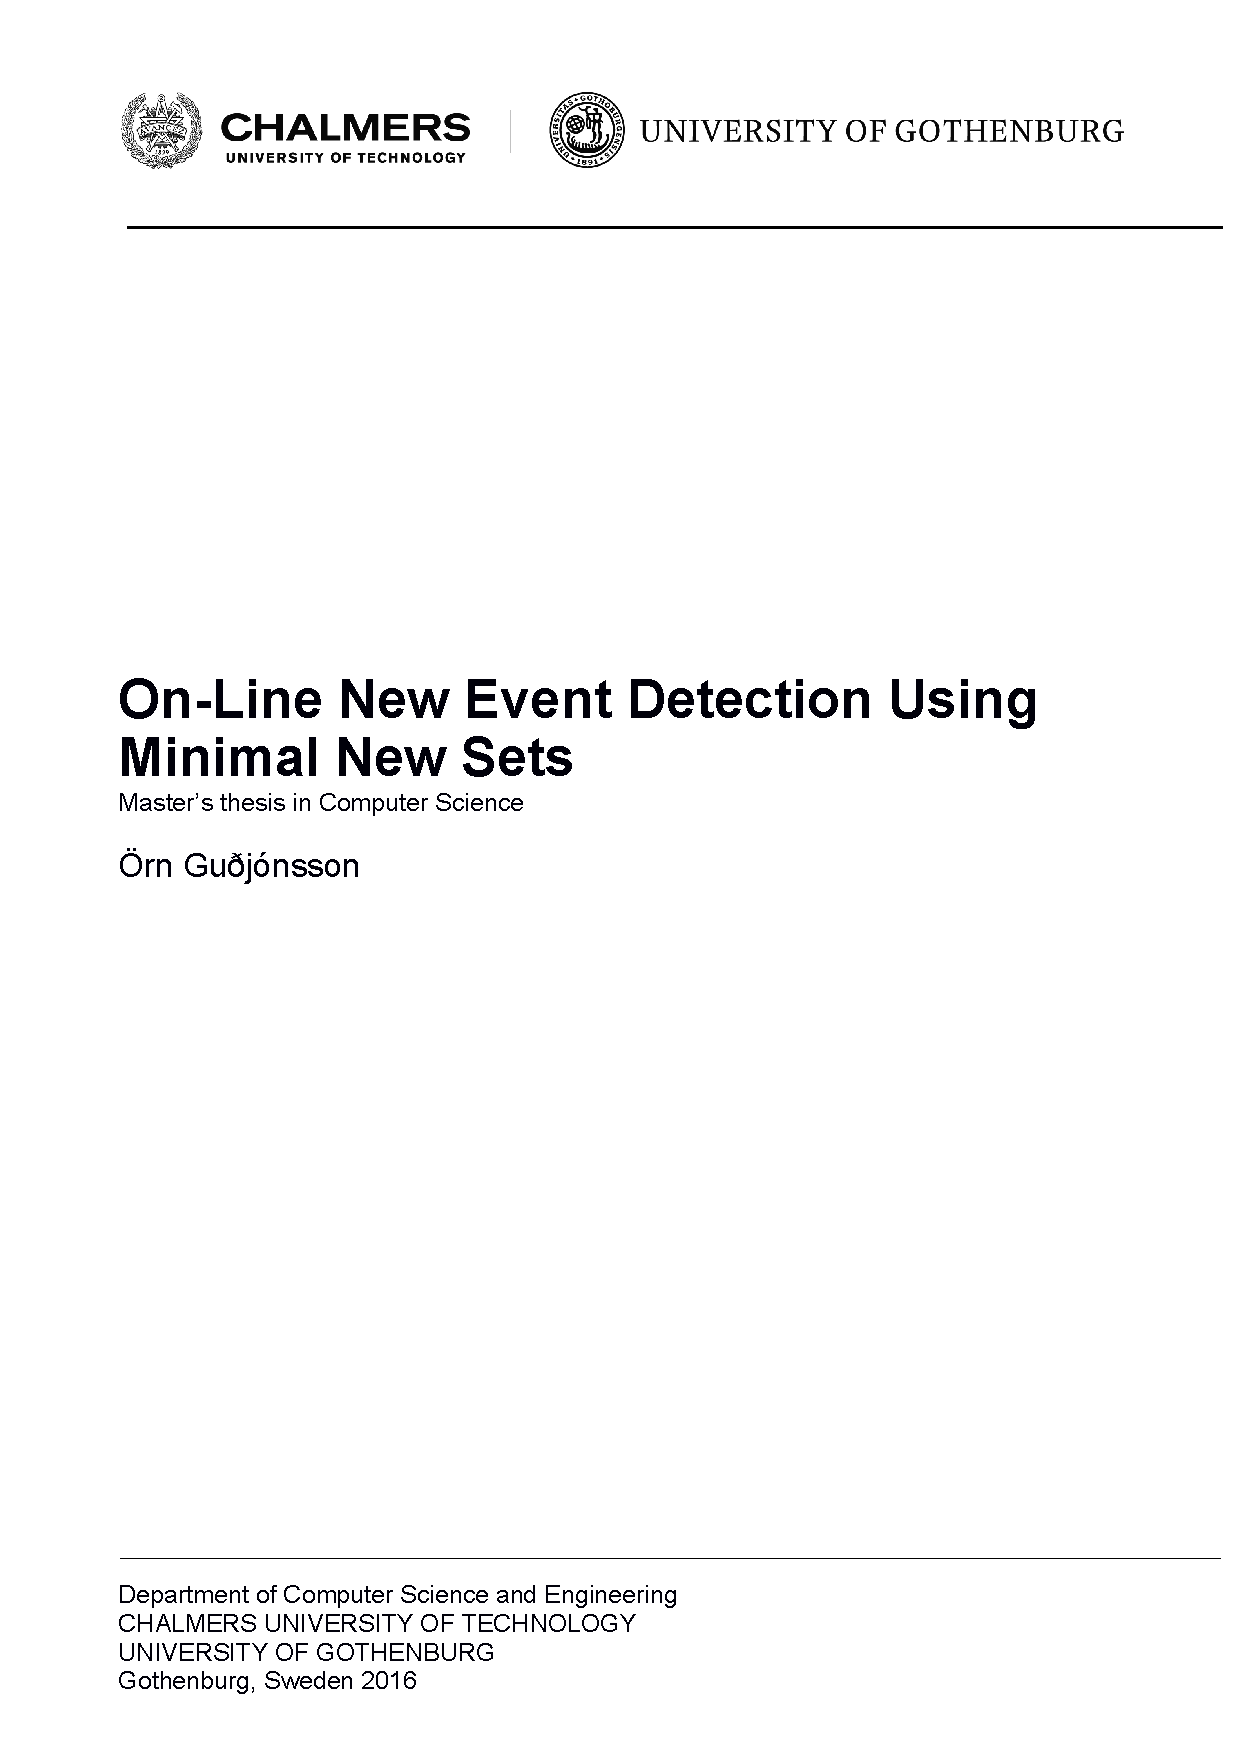
\includepdf[pages={1}]{title/title.pdf}

%\chapter*{Abstract}
%\chapter*{Abstract}
%\label{chapter:abstract}
\begin{abstract}
\emph{On-line New Event Detection} can be used to monitor multiple news streams and determine when a new newsworthy event that might further warrant attention occurs, thus helping the user to not miss out on important information while helping him sift through the vast amount of information available.

In this thesis we present a novel approach for On-line New Event Detection based on computing minimal new sets of small sizes from new stream documents with regards to previously seen documents. We present an algorithm that outputs sets of words likely to be indicative of new events which users easily can browse through and detail several different approaches to select the sets most likely to be informative of new events. In addition we examine the practicality of our approaches and examine the runtime and memory complexities of our algorithms in relation to the most prominent current techniques.
\end{abstract}


%\chapter*{Dedication}
\chapter*{Acknowledgements}
\thispagestyle{empty}
I'd like to thank my supervisor, prof. Peter Damaschke, for the idea for this project and assistance and insights throughout the course of this project.

I'd also like to thank my family for supporting and encouraging me throughout the course of this project. I would especially like to thank my wife, Elfa Björk, for her patience and support without which this thesis would never have been completed.

\clearpage

%To mum and dad

%\chapter*{Declaration}
%I declare that..

%\chapter*{Acknowledgements}
%I want to thank...

\tableofcontents

\chapter{Introduction}
\label{chapter:introduction}
In today's society the amount of information available is vast. The internet, one of the largest sources of information available today, makes finding information easy. Although large parts of the internet consist of images and videos of cats doing silly things there are still numerous sources with structured text information streams, such as news. However, the number of available news streams is so vast that no man is capable of digesting them all. Moreover, the various news sources tend to re-iterate upon events previously reported by themselves or other sources. It can therefore become tedious to try and stay on top of the news. 
Within several domains, such as stock trading, it can be of vital importance to be able to identify important events as soon as they occur and thus the availability of fast and reliable computer systems that aid in the detection of such events can be of great benefit. 

%Over the last few decades the amount of electronically available information has grown rapidly. The daily amount of information that is uploaded to sources such as the internet is so vast that it has become impossible for any human to process it all and keeping track of important events can be overwhelming. 

\emph{On-line New Event Detection} (ONED) is the process of monitoring text information streams and detecting stories that report about new events. For instance, a story reporting a large oil leakage in the Pacific Ocean should be identified as a new story the first time that the event is reported, while consecutive stories further iterating upon the event or stories discussing the environmental effects of the spill should be identified as not containing new events. 

In this thesis we present a new approach to ONED, built upon the concept of identifying minimal new sets of words from new articles and using those as basis for determining whether or not the text refers to a new event. This concept has previously been proposed by Damaschke~\cite{damaschke2015pairs} and Wurzer et al.~\cite{wurzer2015kterm}. The intuition is that when a new event occurs, like the death of a celebrity, we are likely to find words together within the same article that have never occurred before. Moreover we are likely to find small sets of words that have never previously occurred together. For instance, the first report of the recent death of the artist Prince would likely have been the first time the words ``Prince'' and ``dies'' appeared together. By finding and filtering these minimal new sets to only include informative word combinations based on quantitative criteria we are able to present likely events succinctly which allows a user to browse through them.

Unfortunately, finding cases where the aforementioned example fails is trivial. Consider the sentence: ``On Mondays I listen to Prince. On Tuesdays I play Candy Crush until the battery in my phone dies''. Here the words ``dies'' and ``Prince'' occur together without any relation to each other and the pair of them does in this case not indicate any new event. Moreover, if this co-occurrence of these two words would appear before any reports of Prince's death then this would prevent them from being recognized as a new pair in those later reports. Irrelevant co-occurrences could thus yield both false positive and false negatives. In this thesis we explore a few methods which aim to prevent this scenario such as considering the distance between the words and filtering words by importance.

We will start this thesis off by discussing the background of ONED and related works on the topic in chapter~\ref{chapter:background}. We then go through the goals and details of our method in chapter~\ref{chapter:method}. In chapter~\ref{chapter:experiments} we explain the details of our implementation used for the testing and the methods we employ for testing. Chapter~\ref{chapter:results} presents the results of the tests. Finally, in chapter~\ref{chapter:discussion} we discuss our findings and present suggestions for future work.

\chapter{Background}
\label{chapter:background}

The task of detecting new events within a stream of documents can be separated into two camps \emph{Retrospective Event Detection} and \emph{On-line New Event Detection}.Retrospective Event Detection focuses on discovering previously unidentified events from a finite collection of articles~\cite{yang1998study}. On-line New Event Detection (ONED), which is sometimes known as either simply \emph{New Event Detection} (NED) or \emph{First Story Detection} (FSD), instead deals with the problem by trying to identify new events in real-time as soon as they are arrive from live news feeds.

On-line New Event Detection has seen much development in the past 15 years as it has been one of the topics covered by the \emph{Topic Detection and Tracking}(TDT) research program (TODO:missing citation). In this chapter we will present a brief overview of the techniques used for ONED by other researchers within the field.

\section{What are events?}
The concept of events in daily speech can be somewhat ambiguous~\cite{papka1999online} and in order for us to reason about events it is important that we specify what we mean. "The United States invade Vietnam" could be considered an event but at the same time the whole Vietnam War could be considered an event. We use TDT's definition of events: An event is ``a particular thing that happens at a specific time and place, along with all necessary preconditions and unavoidable consequences''. [TODO: cite https://catalog.ldc.upenn.edu/docs/LDC2006T19/TDT2004V1.2.pdf]
A new news-story does therefore not necessarily report an new event. For instance a news story reporting about a natural disaster would contain a new event, whereas consecutive articles detailing the extent of the damage cause and the particulars of the rebuilding efforts that follow, would not. In ONED we want to be able to detect only those stories which contain events, and in particular, only new events which have not been reported before.

\section{Related works}
A classical approach to ONED is to represent documents as term vectors where each term within a document is weighted using some metric, typically TF-IDF (term frequency-inverse document frequency)[TODO: citation], which are then compared in some way to the vector representations of previously seen documents.

Papka, Allan and Lavrenko~\cite{papka1998online} use a single-pass clustering technique where feature extraction and selection techniques are used to build query representations of all stories. They then compare any incoming document to the previously seen queries and flagging the document as new if it's comparison score exceeds a threshold which is calculated for each document.

Yang, Pierce and Carbonell~\cite{yang1998study} also use a single-pass clustering algorithm and incremental IDF for TF-IDF weighting: IDF is first trained on a dataset an then updated for each document. In order to increase efficiency and due to the temporal nature of events they use a sliding time-window to only compare incoming documents to stories within the time window. Additionally they also examine decay weighting where documents further away in time are marked as less important.

Brants, Chen and Farahat~\cite{brants2003system} use a source-specific TF-IDF model where the news stream is comprised out of multiple sources and certain words are more common depending on the source. Each incoming document is weighted and compared to previously seen documents using either Hellinger- or cosine-distance but normalized by subtracting the average distance of the current document to all other documents. [TODO: more stuff that they do]

Another popular approach is to represent documents using named entities. The intuition being that events can be summarized  by ``what'', ``where'', ``when'' and ``how'' and other similar properties. [TODO: citation]

Yang et al.~\cite{yang2002topic} use a supervised learning algorithm to classify documents in an on-line document stream into pre-defined topic categories. Weighting is done using named entities. They then do topic specific stopword removal and topic sensitive feature weighting.

Kumaran and Allan~\cite{kumaran2005using} use named entities in addition to term vectors with incremental TF-IDF weighting as well as topic terms and compute the cosine similarities of each of those features to previously seen documents. A Support Vector Machine (SVM) classifier is then trained on each of those three features.

%TODO: add something about zhang: New Event Detection Based on Indexing-tree and Named Entity

%TODO: add something about li, tao and fu: a new onlien new event detection algorithm based on event merging and event splitting

Petrovic, Osborne and Lavrenko~\cite{petrovic2012using} paraphrase incoming articles and use locality-sensitive hashing for comparisons. 

Wurzer, Lavrenko and Osborne~\cite{wurzer2015kterm} present a constant time/space algorithm for ONED. Their approach is based around finding sets of up to $k$ terms for incoming documents and estimating novelty as the proportion of such sets that have not appeared before. They store subsets of size up to $3$ using a Bloom filter~(TODO: CITATION) with a 32-bit Murmur-hash~(TODO: CITATION). For the Bloom filter they use a fixed-length bit array. This allows them to perform lookups and updates in constant time as well as constant space. To limit the amount of false positives reported by Bloom-filter lookups they zero out a random bit each time the proportion of non-zero bits exceeds a given threshold. This of course means that they forget some of the sets of words that they have seen.

\chapter{Method}
\label{chapter:method}
On-line new event detection is hard~\cite{allan2000hard}. In this chapter we present a new method for ONED based around the concept of \emph{minimal new pairs}. We explain the rationale behind the idea, give a detailed explanation of the base algorithm and discuss some of the approaches we have examined for expanding upon the base idea.


\section{The basic idea}
\label{section:idea}
Damaschke~\cite{damaschke2015pairs} observed that for new articles, the existence of previously unseen small sets of words could be good indicators for new events and presented an efficient algorithm for finding such sets. This is similar to the approach used by Wurzer et al.~\cite{wurzer2015kterm} except they use the proportion of new such sets to quantify the novelty of the novelty of incoming articles while our approach focuses on the new sets themselves and the terms within them. However, the base principle is the same: the first report of Prince's death is likely to be the first document within the stream containing the words ``Prince'' and ``dead'' or similar. 

In more formal terms, Damaschke~\cite{damaschke2015pairs} presents the definition of \emph{minimal new sets}. 

\begin{definition}
  Let $B_0, B_1, B_2...B_{m-1}$ be a sequence of sets that we call bags. For another bag $B:=B_{m}$ we call a subset $X \subseteq B$ new at $m$, if $X$ was not already a subset of an earlier bag : $\forall i < m : X \setminus B_{i} \neq \emptyset$. Otherwise $X$ is said to be old at $m$. We call $X \subseteq B$ minimal new at $m$ if $X$ is new and also minimal (with respect to inclusion) with this property.
\end{definition}

Thus, to continue with our previous example, if we tokenize incoming news articles into bags of words, then $\{prince, dead\}$ would likely be a minimal new set for the first article reporting the tragic event of Prince's death.

A first, naive approach could be to simply base the detection of new events on the existence of minimal sets below a given set size $k$. For example, if we choose $k=3$ we would say that if an article contains new words or new pairs of old words it contains a new event, otherwise it does not. This naive approach does not work well in practice however since articles covering the same event are quite likely to contain new words or new pairs and thus this method is likely to falsely flag articles as containing new events.

Instead of blindly flagging articles based on the existence of minimal sets we propose a method which automatically highlights and presents important informative word combinations by certain quantitative criteria such that the user can then quickly browse them and see which of them raise interest. This introduces the problem of having to prioritize the minimal sets identified for any incoming article.

\section{Enumeration}
\label{method:enumeration}
Central to our approach is the enumeration of incoming articles into, i.e. identifying the minimal new sets. Luckily, Damaschke~\cite{damaschke2015pairs} presents an effective way to enumerate articles:

%In the first pass we look for new words by looking up each word in the bag in some sort of efficient datastructure such as a hashmap. If the word is not found during lookup we store it along with the number of the article that we are currently processing. We also conclude that the word is new. If the word is found during lookup we know that we have encountered it before. From the value stored along with it we also know when it was first encountered. 
%Once we have processed all the words in the bag we potentially have a set of new words which we can compare with the bag. We remove these before the second pass in which we construct all possible sets containing two distinct words from the words that are left in the bag. Next we lookup each of the pairs we've identified in the same manner as before. However, if lookup comes up empty we now have to check that the words in the pair didn't appear together in an article when at least one of them appeared for the first time. Thus, for each of the words in the set we perform a lookup and if the words is found we check if our pair is a subset of the bag in which that word was first encountered. If we can find a bag where the pair is a subset then the pair is not new in the current input article. If no such bag can be found however, then we can conclude that the pair is a minimal new subset of size 2. 
%We now remove all pairs we have identified as new from the bag of pairs and recognize this as the end of the second pass.
%If there are any pairs left we find all subsets of size 3 from the bag of pairs and proceed in the same way until there are the bag is empty at the end of a pass. 

Let's say that at time $m$ we have stored the bags of previous articles sequentially: $B_0, B_1, B_2...B_{m-1}$. In order to find all minimal new sets of bag $B_{m}$ we generate candidate sets $X \subset B_{m}$ of increasing sizes until all candidates are supersets of already discovered minimal new sets. First we find all, if any, words that are new at $m$, then from any words that are not new at $m$ we find all possible sets of size 2 (pairs) and check for each of them if they are new at $m$. If there are any pairs that were not new at $m$ we find sets of size 3 from those, etc. 

The key to making the algorithm efficient lies in how we determine whether a set $X$ is new at $m$. We create a function, $f$ so that $f(X) := min\{i \mid X \subseteq B_{i}\}$ and let $f(X)$ be undefined if $X$ is not a subset of any bag $B_{i}$. Now $X$ is new at $f(X)=i$ if such a value exists, and old at any subsequent index $j>i$. 

When enumerating bag $B_{i}$ we store $X$ along with $f(X)=i$ for each of the candidate sets that we determine to be minimal new at $i$. For any set of size 1 we can easily determine if it is a minimal new set simply by checking whether a value for that set has been stored in the table.  Any time that a word makes it first appearance any larger subset of words from the same bag containing that word will also be new at that time, but not minimal. For any larger candidate set $X \subseteq B_{m}$, $|X|>1$ we therefore might have to take further steps to determine whether $X$ is new at $m$. Again, if $f(X)$ is stored we know that $X$ is old. If $f(X)$ is not stored then for each $Y \subset X$ we check if $f(Y)$ is stored. If $f(Y)=j$ is stored then we check if $X \subset B_{j}$. If such a $j$ is found then $X$ was new at $j$ but is old at $m$. If no such $m$ is found we conclude that $X$ is new at $m$.


\section{Pre-processing}
Prior to extracting the minimal sets from an article the article must be preprocessed so that we can digest it. For our enumeration algorithm [TODO: ``enumeration'' is explained in Damaschke2015 but we must also explain it here before we talk about it] we treat articles as sets of words, \emph{bags}, and therefore we must pre-process any article that we receive as input before we can enumerate it and apply any of our methods. We tokenize the input articles, remove stopwords and punctuation and stem the tokenized words using the English porter2 stemmer provided by the NLTK. [TODO: add citation for NLTK and porter2]

\section{Approaches}
As explained in section~\ref{section:idea} we have to filter out or select from the minimal sets that we identify within incoming articles in order to be able to present the informative sets that are likely to be indicative of a new event. In this section we will discuss the approaches we examined in order to try to accomplish this: filtering common or unimportant words, prioritizing words that occur in many minimal new pairs, prioritize words that appear with close proximity.

\subsection{Filtering common or unimportant words}
Words which describe a new event are likely to be relatively unique to that event. Reversely, words which are common over multiple different articles are likely to not be descriptive for new specific events. [TODO: citation?] Similarly, words which are common within an article are likely to be important for that article. Thus, we suggest filtering out words that are common within the previously seen articles, or words which can be determined not to be important within the incoming article. Thus we can filter based on \emph{collection frequency}: how often a given word has appeared within the accumulated corpus; \emph{document frequency}: the number of documents in which a given word has previously appeared; the \emph{TF-IDF} score: a score indicating the importance of a word within the given article with relation to how common it is within the corpus.

\subsection{Prioritizing words that occur in many minimal new pairs}
An article reporting a new event is likely to contain many new pairs of words that previously have not appeared together. [TODO: citation?] Commonly used words are however likely to have appeared together. Thus, minimal new sets of size $>1$ are likely to contain at least one word that is more indicative of the events described within the given article. If a particular word can be found within a majority of the minimal new sets, then it is likely to be an old word within a new context and likely to be a key property of the article. For instance, the words ``purple'', ``rain'' and ``Prince'' are likely to have appeared together before in Prince related articles. An article that then yields the minimal new sets $\{Prince, dead\}, \{purple, dead\}, \{rain, dead\}$ gives us a  common denominator in ``dead'' within the minimal set, indicating that ``dead'' is likely to be an important indicator of a possible new event. Based on this idea we can identify important words by counting the number of minimum new sets they appear in. In particular we focus on prioritizing words that occur in many minimal new pairs.

\subsection{Prioritizing words that appear in close proximity}
Words that are indicative of new events are likely to be find in close proximity. For instance an article reporting about a volcanic eruption at Yellowstone is much more likely to contain something along the lines of ``Volcanic eruption at Yellowstone'' than mentioning ``Yellowstone'' in one paragraph and ``eruption'' several paragraphs later.

For any minimal new sets of an article we can calculate the minimum amount of words between the elements within the sets and find which sets contain words which occur close to each other within the article. Using this we can prioritize sets of words which appear more closely together within the article in the hopes that they are good indicators of potential events.

\subsection{Splitting articles into smaller parts}
Another approach for increasing the importance of words that appear together is to split an article into several smaller, sub-articles. Some natural examples of such sub-articles would be paragraphs or either sentences. One can easily imagine that important event-related words appear within the same paragraph or even the same sentence. This requires an extra pre-processing step: splitting up incoming articles into the wanted bits. In addition this requires some trivial changes to the base algorithm. For each article we have to feed each sub-bag to our algorithm but take care not to add any words to the list of previously seen bags until after we have processed all the sub-bags of the incoming article so as to avoid identifying words that first appear within the given article as old in sub-bags which are subsequent to the sub-bag in which they first appear.

Let the sub-bags $P_{k} := [S_{0}, S_{1},...,S_{q}]$ be a list of the sub-bags generated from article $k$ so that for the bag of all the words in the article $B_{k}$ it holds that $\bigcup_{i=0}^{q}S_{i} = B_{k}$. We call $P_{k}$ the parent bag for article $k$. We assume that we have stored all the previous parent bags $S_{0},...,S_{k-1}$ as well as mappings from all previously minimal bags to sub-bags within parent-bags. The enumeration of $B_{k}$ is now the union of the all the enumerations of the sub-bags $S_{i} \mid i \in [0,q]$ where each $S_{i}$ is enumerated using the approach described in section~\ref{method:enumeration}. If a minimal new set $X$ is found while processing sub-bag $S_{i} \in P_{k}$ we store the minimal new set along with both the numbers $k$ and $i$. If the same set $X$ is found in another sub-bag $S_{j} \in P_{k}$ where $j>i$ we need to make sure to store $j$ as well. We let $f'(X)$ be a function which returns the number of the  parent-bag in which $X$ was minimal new as the sub-bags of that bag which contained $X$. In other words we store $f'(X) = (k, [i,j])$, to indicate that $X$ was minimal new at $k$ and found in sub-bags $i$ and $j$. 

Just like in the original enumeration algorithm, we don't have to rely on naive exhaustive search to calculate $f'(X)$ for any $|X|>1$. For each $Y\subset X$ we can lookup $f'(Y)$ and if a pair $(k, [l_{0}... l_{q}])$ is found we check $X \subseteq S_{k, i} \mid S_{k, i} \in P_{k}, i\in[0,q]$. If such a $S_{k,i}$ is found we know that $X$ is old. Furthermore we can conclude that $X$ was new at the smallest $k \mid f'(Y)=(k, [l_{0},..., l_{q}])$.

\subsubsection{Joining sub-bags}
Using the same idea we can create a ``sliding window'' of $k$ sub-bags to increase the sizes of the sub-bags and thus increasing the odds of finding new combinations of words. A simple example would be to always use three consecutive sentences as sub-bags when available. Thus the first three sentences of an article would make up a sub-bag, then the second to the fourth sentence would make up the next sub-bag etc. For each consecutive sentence the first sentence of the previous bag would be removed and the new sentence added, like sliding a three-sentence wide window over the article. This approach allows us to explore larger sub-bags while preventing us from missing important word combinations which we could miss if we were to simply choose the first three sentences followed by the next three etc.

\chapter{Experiments}
\label{chapter:experiments}
TODO: explain in detail out implementations, approaches tested, how we tested and on what datasets, how the datasets were obtained etc.

We implemented the concepts discussed in chapter~\ref{chapter:method} using the Python (TODO: CITATION) programming language. We then used these implementations to test the effectiveness of the various methods on several different datasets. In this chapter we discuss our implementation in some detail as well as how the tests were carried out along with what data was used for testing.

\section{Implementation}
For our implementation we chose Python because it supports many high-level concepts such as lamda functions, list comprehensions etc. as well as for its extensive standard library and excellent availability of good third-party libraries such as the Natural Language Tool Kit (NLTK) (TODO: CITATION).

\subsection{Pre-processing}
The NLTK provided us with most of the parts needed for preprocessing: we used the built-in word-tokenizer for splitting whole-string articles into lists of words,  stopwords from the English corpus for stopword-removal and the porter2 stemmer for fast and simple stemming of words. Python's string module provided us with a list of punctuation characters which we used to remove punctuation. Our pre-processing step first removed any punctuation character, then tokenized the input-string, removed all the stopwords then stemmed each of the tokens. (TODO: CITATIONS? PORTER2, nltk)

\subsection{Enumeration}
We have implemented the algorithm described in section~\label{method:enumeration}. Our implementation uses sets of strings (or Python's frozensets in cases where the sets had to be hashed) to represent the bags of words to enumerate, a list of bags (list of sets of strings) to store previously seen bags and a dictionary (hashmap) with frozensets as keys and integers as values for mapping previously seen minimal new sets to the number of the bag in which they first appeared.

\section{Tests}
We conducted several series of tests on various data sources. The different configurations and approaches which we tested were:

\emph{Configuration-1}: The base algorithm without any further analysis or filtering of the input and output sets beyond the basic pre-processing described in section~\ref{method:preprocessing}. Additionally, we conducted experiments with sorting new pairs in descending order based on the minimum distance between the words in the pairs or the combined number of minimal-new sets that the words appeared in. In the latter case we also outputted the number of minimal-new sets the words appeared in.

\emph{Configuration-2}: Simple output filtering using either TF-IDF, document frequency or collection frequency by only outputting sets which contained at least one words with a score above the given filtering threshold. 

\emph{Configuration-3}: The same as Configuration-2 except filtering picked the words with the $k$ highest scores, where $k$ was the given threshold value. Tested with several different values of $k$.

\emph{Configuration-4}: Configuration-2 but applying filtering prior to enumeration.

\emph{Configuration-5}: Configuration-3 but applying filtering prior to enumeration.

\emph{Configuration-6}: Enumerating articles by splitting them into sub-bags where each sub-bag was either a sentence, a paragraph or a sliding window of $k$ consecutive sub-bags for different values of $k$.

\emph{Configuration-7}: Normal enumeration with filtering by including the $k$ highest TF-IFD scoring words like in Configuration-3 combined with filtering pairs to only include those who's words had a combined TF-IDF score above some provided threshold.

\emph{Configuration-8}: Like Configuration-7 but using sub-bags for enumeration, either based on sentences, paragraphs or a sliding window.

Each configuration was tested with several different parameters on real data obtained by crawling various sources for on-line news. The crawled articles were stored along with their dates of publication so that they could later be consumed in the same order that they would have arrived should they have been processed by an on-line news monitoring system. For each digested article the original article was printed along with the output of the enumeration and later evaluated. 

\subsection{Evaluation}
Since we have not yet found a good quantification method for performing automatic New Event Detection we evaluated the results of our test runs manually by comparing the outputs of the various configurations. In particular we were interested in finding methods which prioritized minimal new sets which captured the main points of the input articles. 

\subsection{Data}
All of the data that we used for testing was real data obtained from various sources from the internet, they contained articles of various types and lengths since we also wanted to identify to some extent for what type of input the approaches where successful. The datasets we used were:

\emph{D1}: A collection of very short summary articles and headlines collected from articles regarding the 2016 presidential election in the USA, gathered from pbs.org, reuters.com and cbsnews.com (TODO: CITATIONS!). The data was gathered on 04.04.2016 containing articles published on dates ranging from 03.03.2016 to 04.04.2016 (TODO: HOW MANY ARTICLES?). This dataset served to test our approach on short articles within a narrow topic. Our hope was that short articles within a shared topic would provide good results, since high word density within a shared topic combined with the low overall word count of each article would decrease the amount of new words found and instead yield interesting new pairs.

\emph{D2}: Timelines of president Barack Obama's years of presidency, '09, '10 and '11, taken from wikipedia.org (TODO: citation). Similar to D1 each point of the timeline can be regarded as a very short article and in this case is very likely to refer to an event. The data was gathered on (TODO: DATE!).

\emph{D3}: A chronological account of the events of the second war taken from (TODO: CITATION!) where we treated each paragraph as a separate article. The point of this dataset was to test our approaches on slightly longer and less densely focused articles within a single topic. The data was gathered on (TODO: DATE!).

\emph{D4}: Real life full-length news articles taken from reuters.com (TODO: CITATION!). The data was gathered on 03.08.2016 and includes articles dating from 04.11.2016-03.08.2016. The purpose of this dataset was to simulate real-life usage of an ONED system on a large set of data.

\chapter{Results}
\label{chapter:results}
In this chapter we will look at the results of the experiments discussed in chapter~\ref{chapter:experiments}.

\Crefrange{tab:d1}{tab:d4} show the ratio of articles which resulted in no new words, no new pairs or both. In the cases where filtering was applied a shorthand for the filter type (cf=collection frequency, tf=term frequency) is included as well as the threshold. We noted that filtering did in fact increase the number of empty output-sets of either size and in the cases of the collection frequency and term frequency filters along with any pre-enumeration filtering (Configuration-3) the change was quite drastic.

\begin{center}
\begin{table}
  \begin{tabular}{|l|c|c|c|}
    \hline
    &  No new words & No new Pairs & Both \\ \hline
    Configuration-1                    & 0.04  & 0.03  & 0.01 \\ \hline
    Configuration-2 (cf: 5)            & 0.00  & 1.00  & 0.93 \\ \hline
    Configuration-2 (tf: 5)            & 0.58  & 0.42  & 0.41 \\ \hline
    Configuration-2 (tfidf: 5)         & 0.05  & 0.35  & 0.01 \\ \hline
    Configuration-3 (cf: 5)            & 0.19  & 0.92  & 0.85 \\ \hline
    Configuration-3 (tf: 5)            & 0.01  & 0.99  & 0.96 \\ \hline
    Configuration-3 (tfidf: 5)         & 0.00  & 0.74  & 0.01 \\ \hline
    Configuration-4                    & 0.04  & 0.03  & 0.01 \\ \hline
    Configuration-4 (tfidf: 5)         & 0.04  & 0.52  & 0.02 \\ \hline
  \end{tabular}
  \caption{The outcomes from running different configurations on dataset D1}
  \label{tab:d1}
\end{table}
\end{center}

\begin{center}
\begin{table}
  \begin{tabular}{|l|c|c|c|}
    \hline
    &  No new words & No new Pairs & Both \\ \hline
    Configuration-1                    & 0.10  & 0.01  & 0.00 \\ \hline
    Configuration-2 (tfidf: 5)         & 0.12  & 0.25  & 0.00 \\ \hline
    Configuration-3 (tfidf: 5)         & 0.01  & 0.69  & 0.00 \\ \hline
    Configuration-4                    & 0.10  & 0.01  & 0.00 \\ \hline
    Configuration-4 (tfidf: 5)         & 0.11  & 0.36  & 0.01 \\ \hline
  \end{tabular}
  \caption{The outcomes from running different configurations on dataset D2}
  \label{tab:d2}
\end{table}
\end{center}

\begin{center}
\begin{table}
  \begin{tabular}{|l|c|c|c|}
    \hline
    &  No new words & No new Pairs & Both \\ \hline
    Configuration-1                    & 0.16  & 0.10  & 0.01 \\ \hline
    Configuration-2 (tfidf: 5)         & 0.16  & 0.30  & 0.01 \\ \hline
    Configuration-3 (tfidf: 5)         & 0.11  & 0.55  & 0.01 \\ \hline
    Configuration-4                    & 0.16  & 0.10  & 0.01 \\ \hline
    Configuration-4 (tfidf: 5)         & 0.16  & 0.32  & 0.01 \\ \hline
  \end{tabular}
  \caption{The outcomes from running different configurations on dataset D3}
  \label{tab:d3}
\end{table}
\end{center}

\begin{center}
\begin{table}
  \begin{tabular}{|l|c|c|c|}
    \hline
    &  No new words & No new Pairs & Both \\ \hline
    Configuration-1                    & 0.13  & 0.74  & 0.13 \\ \hline
    Configuration-2 (tfidf: 5)         & 0.23  & 0.74  & 0.65 \\ \hline
    Configuration-3 (tfidf: 5)         & 0.18  & 0.65  & 0.33 \\ \hline
    Configuration-4                    & 0.18  & 0.64  & 0.08 \\ \hline
    Configuration-4 (tfidf: 5)         & 0.32  & 0.64  & 0.55 \\ \hline
  \end{tabular}
  \caption{The outcomes from running different configurations on dataset D4}
  \label{tab:d4}
\end{table}
\end{center}

One of the events touched upon in the D2 dataset is the BP-oil spill in the Gulf of Mexico\footnote{\url{https://en.wikipedia.org/wiki/Deepwater_Horizon_oil_spill}} and president Obama's actions revolving that incident. \Crefrange{lst:original}{lst:config6} show the enumerations of an article in which the event was mentioned for the second time, enumerated using different configurations. In this case the event would be that president Obama answered questions regarding the oil spill.

As is to be expected, the enumerations using Configuration-2 and Configuration-4 are very similar since most of the articles in the dataset only contain one sentence and therefore only one sub-bag. Apart from the enumeration generated by Configuration-3 which contains no useful insights about the contents of the article, the generated enumerations appear to capture the main gist of the article. For configurations 1,3 and 4 the minimal new sets have been sorted based on TF-IDF score, in descending order. 

%In \cref{tab:nodeCounts} we show the number of different new pairs in which the involved words occurred. We observe that in this case words which appear in many new pairs appear to have high significance within the article.

\begin{lstlisting}[frame=single,
    caption=Original text,
    label={lst:original},
  ]
  May 27  – President Obama holds a news conference in the East Room to answer questions about the  BP  Deepwater Horizon  Gulf of Mexico oil spill . 
\end{lstlisting}

\begin{lstlisting}[frame=single,
    caption=Configuration-1,
    label={lst:config1},
  ]
New Words: {deepwat, horizon}
New Pairs: {(question, bp), (spill, question), (gulf, bp), (spill, answer), (bp, answer), (gulf, question), (gulf, spill), (question, news), (bp, news), (spill, news), (gulf, answer), (question, oil), (mexico, question), (mexico, bp), (mexico, spill), (spill, 27), (question, 27), (bp, 27), (answer, news), (gulf, news), (question, east), (bp, east), (spill, east), (bp, confer), (spill, confer), (question, confer), (question, room), (bp, room), (spill, room), (question, may), (spill, hold), (bp, hold), (question, hold), (oil, answer), (mexico, answer), (gulf, 27), (27, answer), (oil, news), (east, answer), (confer, answer), (gulf, confer), (room, answer), (gulf, room), (mexico, news), (gulf, may), (may, answer), (gulf, hold), (27, news), (east, news), (room, news), (may, news), (oil, 27), (confer, oil), (mexico, 27), (room, oil), (oil, hold), (mexico, confer), (east, 27), (mexico, room), (confer, 27), (mexico, hold), (room, 27), (27, may), (east, may)}
\end{lstlisting}

\begin{lstlisting}[frame=single,
    caption=Configuration-2,
    label={lst:config3},
  ]
New Words: {deepwat, horizon}
New Pairs: {(question, bp), (spill, question), (gulf, bp), (spill, answer), (bp, answer), (gulf, question), (gulf, spill), (question, news), (bp, news), (spill, news), (question, oil), (mexico, question), (mexico, bp), (mexico, spill), (spill, 27), (question, 27), (bp, 27), (question, east), (bp, east), (spill, east), (bp, confer), (spill, confer), (question, confer), (question, room), (bp, room), (spill, room), (question, may), (spill, hold), (bp, hold), (question, hold)}
\end{lstlisting}

\begin{lstlisting}[frame=single,
    caption=Configuration-3,
    label={lst:config5},
  ]
New Words: {horizon, deepwat, question}
  New Pairs: {}
\end{lstlisting}

\begin{lstlisting}[frame=single,
    caption=Configuration-4,
    label={lst:config6},
  ]
New Words: {deepwat, horizon}
New Pairs: {(question, bp), (spill, question), (gulf, bp), (spill, answer), (bp, answer), (gulf, question), (gulf, spill), (question, news), (bp, news), (spill, news), (question, oil), (mexico, question), (mexico, bp), (mexico, spill), (spill, 27), (question, 27), (bp, 27), (question, east), (bp, east), (spill, east), (bp, confer), (spill, confer), (question, confer), (question, room), (bp, room), (spill, room), (question, may), (spill, hold), (bp, hold), (question, hold), (question, –)}
\end{lstlisting}

\Crefrange{fig:setPlot1}{fig:setPlot4} show how the amount of minimal new sets of size less than 3 found in enumeration change over time using different configurations. In all cases the amount of new words found decreases over time while the amount of new pairs found tends to increase over time.

\begin{figure}[ht]
  \centering
  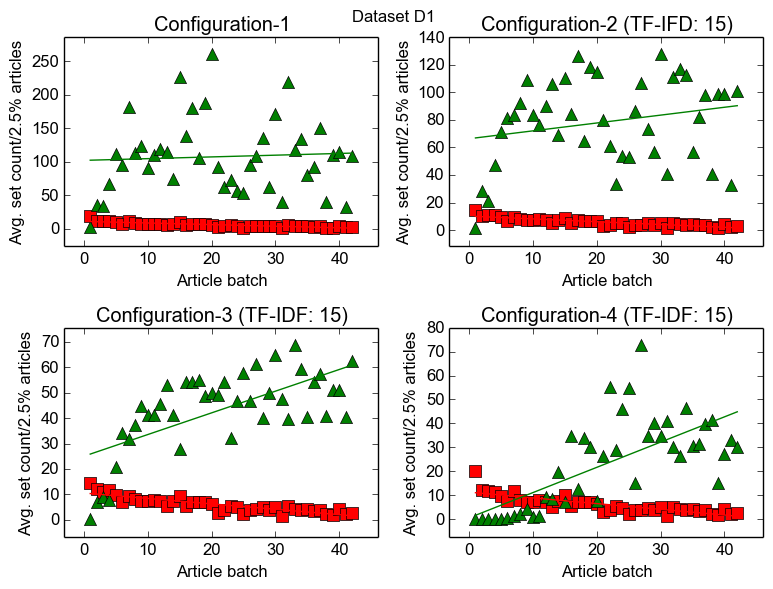
\includegraphics[scale=0.70]{images/D1-plot.png}
  \caption{Average number of new words and new pairs per batch of 2.5\% of all articles in dataset D1}
  \label{fig:setPlot1}
\end{figure}

\begin{figure}[ht]
  \centering
  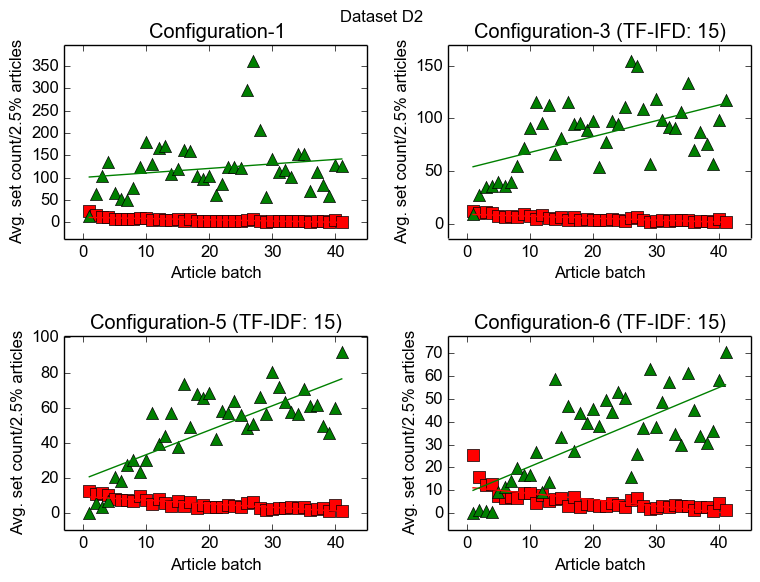
\includegraphics[scale=0.70]{images/D2-plot.png}
  \caption{Average number of new words and new pairs per batch of 2.5\% of all articles in dataset D2}
  \label{fig:setPlot2}
\end{figure}

\begin{figure}[ht]
  \centering
  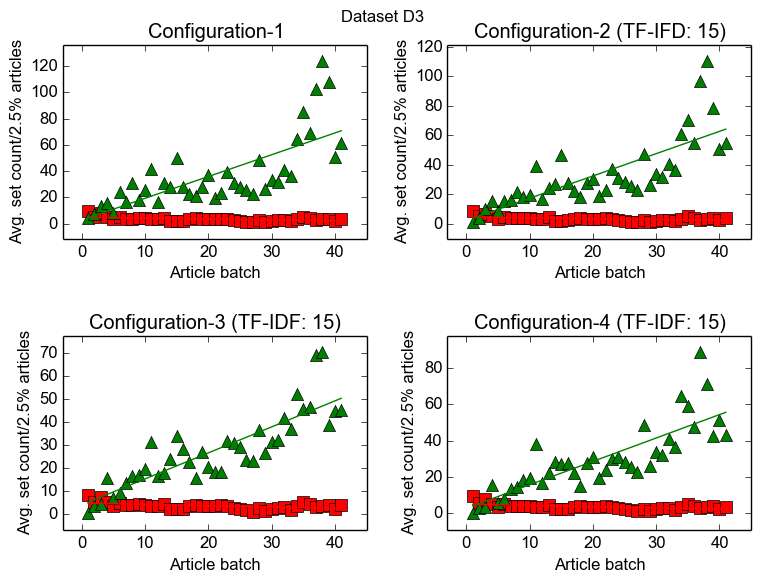
\includegraphics[scale=0.70]{images/D3-plot.png}
  \caption{Average number of new words and new pairs per batch of 2.5\% of all articles in dataset D3}
  \label{fig:setPlot3}
\end{figure}

\begin{figure}[ht]
  \centering
  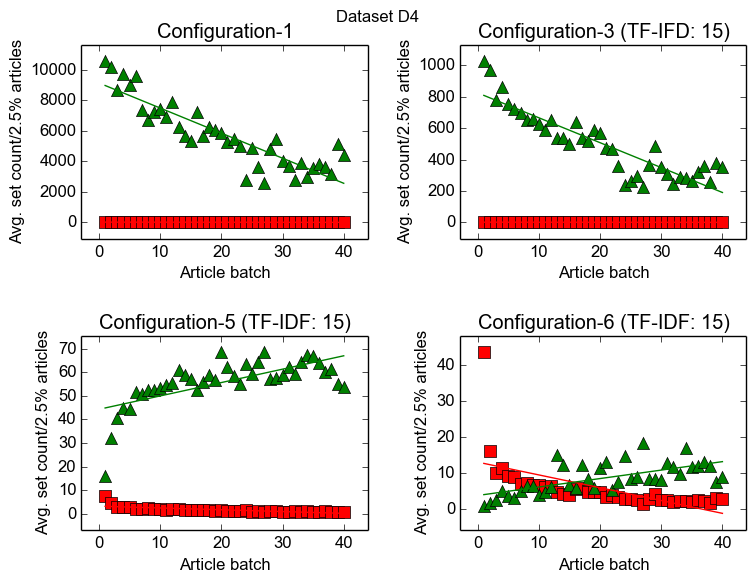
\includegraphics[scale=0.70]{images/D4-plot.png}
  \caption{Average number of new words and new pairs per batch of 2.5\% of all articles in dataset D4}
  \label{fig:setPlot4}
\end{figure}

\section{Benchmarks}
For each configuration we measured the time taken to process each of the datasets. Although each run produced the same output we performed each test 20 times to achieve more accurate benchmarks. \Cref{tab:benchmark1} shows the average time per article for different configurations. \Cref{tab:benchmark2} shows the combined average time per article for the same configurations for configurations using sub-bags and vice versa.

\begin{center}
\begin{table}
  \begin{tabular}{|l|c|}
    \hline
    Configuration & time/article (s)  \\ \hline
    Configuration-1                     & 0.3909 \\ \hline
    Configuration-2 (tfidf: 15)         & 0.2939 \\ \hline
    Configuration-4                     & 0.0533 \\ \hline
    Configuration-4 (tfidf: 15)         & 0.0488 \\ \hline
  \end{tabular}
  \caption{Average runtimes per article using different configurations}
  \label{tab:benchmark1}
\end{table}
\end{center}

\begin{center}
\begin{table}
  \begin{tabular}{|l|c|}
    \hline
    Configuration & time/article (s)             \\ \hline
    Configurations without sub-bags     & 0.3424 \\ \hline
    Configurations with sub-bags        & 0.0510 \\ \hline
  \end{tabular}
  \caption{Average runtimes per article using sub-bags or not}
  \label{tab:benchmark2}
\end{table}
\end{center}

\chapter{Discussion}
\label{chapter:discussion}
The results presented in the previous chapter indicate that minimal-new sets can indeed be good indicators new events or at least novelty within articles. However, simply checking for the existence of minimal new sets containing only one or two elements is not sufficient for determining if an article contains a new event or not and further work has to be done to develop a method to quantify the enumerations to calculate the probability of them relating to a new event.

\Crefrange{fig:setPlot1}{fig:setPlot4} show that over time the amount of new words found decreases while at the same time the amount of new pairs appears to increase. If we are more interested in new pairs than new words then it might therefore be a good idea to pre-train the system on some set of articles so as to skip past the period in which we mostly find new words.

The results of our experiments support our theory that TF-IDF is a good filter to use if we want to decrease the output size, but that filtering should be done on the output rather than the input.

\section{Drawbacks of our approach}
Although it could be argued that our system could be useful for humans to perform tool-assisted New Event Detection where users scan through a small number of minimal new sets for incoming articles and are as such able to process the incoming article faster than they would by reading through them, the system still requires manual labour. In, fact since it is not yet able to perform automatic Event Detection it is not really an ONED-system.

If the enumerations generated by our system could be used as a basis for ONED then there would still be other technical problems to left to solve. 
A weakness of the current enumeration algorithm is events which are repeated or events which occur as history repeats itself, e.g. someone is shot in times square today and then someone else is shot during similar conditions some time later. This later event is a separate and new event, distinct from the first, but is rather likely to not result in any minimal new sets since they would have been introduced by the first shooting.

Since our enumeration algorithm builds up a collection of minimal new sets one can not easily remove old enumerations without sacrificing accuracy since the elements which were minimal-new in the set that is to be removed might have reappeared in a later set and the removal of the first set would therefore require the later set to be update. Because we do not know what sets require updates we would have to traverse all the stored bags which arrived after the set we are removing until we either run out of bags to check or minimal new sets found in the removed enumeration.

Others have developed such systems which forget seen articles over time. Yang, Pierce and Carbonell~\cite{yang1998study} use a sliding window which specifies which previously seen stories they compare incoming stories to. Furthermore they explore weight decay where older stories within the window are given less weight.

As discussed in chapter\ref{chapter:background} Wurzer, Lavrenko and Osborne~\cite{wurzer2015kterm} present an ONED system based on the proportion of subsets up to size $k$, for some small integer $k$, which have not been previously stored. Through the use of a Bloom-filter they are able to operate in constant time per input set in relation to the number of seen articles as well as in constant memory. In their tests they used $k=3$ and achieved impressive results. However, since they do not only consider minimal new sets they always have to find all possible subsets of size $k$ of the incoming bag $B_{n}$ whereas we might achieve faster times, especially for larger values of $k$. We are bounded by \BigO{|B_{n}|\times 2^{k}/k!} while they are bounded by \BigO{|B_{n}|} and since $\lim_{x \to \infty}2^{k}/k!=0$ our approach is better suited for larger values of $k$. 

\subsection{Future Work}
We believe that the results indicate that an effective fully automatic ONED system could be built using our approach of enumerating minimal new sets but different ways for quantifying the enumeration have to be studied. Possible quantification methods might include combining our approach with named entity extraction and using the number of minimal new sets containing named entities as indicators of new events. Another possible approach would be to incorporate the previously discussed technique used by Wurzer, Lavrenko and Osborne~\cite{wurzer2015kterm} and use the ratio of the amount of minimal new sets of size less than some integer $k$ over the amount of possible subsets of size less than $k$. We might be able to achieve better accuracy since we never discard any found minimal-new sets while they flip random bits in the Bloom-filter in order to decrease the probability of false positives.

As we discussed earlier, not being able to forget stories over time might be a drawback. As such the enumeration algorithm would have to be updated in order to allow for that.


\chapter{Conclusion}
\label{chapter:conclusion}
We have presented the basis for a novel approach to ONED based on finding minimal new subsets from incoming news article. Through experiments we have examined the feasibility of such an approach being used for successful ONED. Furthermore we have presented and tested some ideas for further improving the data outputted by the base approach. We believe that the results of our experiments support the idea that minimal new sets could be good indicators of new events within news articles, however further work is required in order be able to use it for fully automatic ONED.


\printbibliography

\appendix 
\chapter{Source Code}
\label{appendix:source}

\section{main.py}
The driver for our implementation.
\inputminted[fontsize=\scriptsize,breaklines]{python}{../src/enumerator/main.py}

\section{bag.py}
The main code for enumeration calculations and bag handling.
\inputminted[fontsize=\scriptsize,breaklines]{python}{../src/enumerator/bag.py}

\section{filters.py}
Contains filter related calculations.
\inputminted[fontsize=\scriptsize,breaklines]{python}{../src/enumerator/filters.py}

\section{preprocessing.py}
Contains code that's used for preprocessing.
\inputminted[fontsize=\scriptsize,breaklines]{python}{../src/enumerator/preprocessing.py}

\section{helpers.py}
Utility functions for printing out results etc.
\inputminted[fontsize=\scriptsize,breaklines]{python}{../src/enumerator/helpers.py}

\end{document}
